\documentclass{beamer}
\mode<presentation>
\usepackage{amsmath}
\usepackage{amssymb}
%\usepackage{advdate}
\usepackage{adjustbox}
\usepackage{subcaption}
\usepackage{enumitem}
\usepackage{multicol}
\usepackage{mathtools}
\usepackage{listings}
\usepackage{url}
\def\UrlBreaks{\do\/\do-}
\usetheme{Boadilla}
\usecolortheme{lily}
\setbeamertemplate{footline}
{
  \leavevmode%
  \hbox{%
  \begin{beamercolorbox}[wd=\paperwidth,ht=2.25ex,dp=1ex,right]{author in head/foot}%
    \insertframenumber{} / \inserttotalframenumber\hspace*{2ex} 
  \end{beamercolorbox}}%
  \vskip0pt%
}
\setbeamertemplate{navigation symbols}{}

\providecommand{\nCr}[2]{\,^{#1}C_{#2}} % nCr
\providecommand{\nPr}[2]{\,^{#1}P_{#2}} % nPr
\providecommand{\mbf}{\mathbf}
\providecommand{\pr}[1]{\ensuremath{\Pr\left(#1\right)}}
\providecommand{\qfunc}[1]{\ensuremath{Q\left(#1\right)}}
\providecommand{\sbrak}[1]{\ensuremath{{}\left[#1\right]}}
\providecommand{\lsbrak}[1]{\ensuremath{{}\left[#1\right.}}
\providecommand{\rsbrak}[1]{\ensuremath{{}\left.#1\right]}}
\providecommand{\brak}[1]{\ensuremath{\left(#1\right)}}
\providecommand{\lbrak}[1]{\ensuremath{\left(#1\right.}}
\providecommand{\rbrak}[1]{\ensuremath{\left.#1\right)}}
\providecommand{\cbrak}[1]{\ensuremath{\left\{#1\right\}}}
\providecommand{\lcbrak}[1]{\ensuremath{\left\{#1\right.}}
\providecommand{\rcbrak}[1]{\ensuremath{\left.#1\right\}}}
\theoremstyle{remark}
\newtheorem{rem}{Remark}
\newcommand{\sgn}{\mathop{\mathrm{sgn}}}
\providecommand{\abs}[1]{\left\vert#1\right\vert}
\providecommand{\res}[1]{\Res\displaylimits_{#1}} 
\providecommand{\norm}[1]{\lVert#1\rVert}
\providecommand{\mtx}[1]{\mathbf{#1}}
\providecommand{\mean}[1]{E\left[ #1 \right]}
\providecommand{\fourier}{\overset{\mathcal{F}}{ \rightleftharpoons}}
%\providecommand{\hilbert}{\overset{\mathcal{H}}{ \rightleftharpoons}}
\providecommand{\system}{\overset{\mathcal{H}}{ \longleftrightarrow}}
	%\newcommand{\solution}[2]{\textbf{Solution:}{#1}}
%\newcommand{\solution}{\noindent \textbf{Solution: }}
\providecommand{\dec}[2]{\ensuremath{\overset{#1}{\underset{#2}{\gtrless}}}}
\newcommand{\myvec}[1]{\ensuremath{\begin{pmatrix}#1\end{pmatrix}}}
\let\vec\mathbf

\lstset{
%language=C,
frame=single, 
breaklines=true,
columns=fullflexible
}

\numberwithin{equation}{section}

\usetheme{Montpellier} 

\title{Collinearity of points}
\author{SRIHAAS GUNDA- EE24BTECH11026}
\date{}


\begin{document}

\frame{\titlepage} 

\begin{frame}{Question}
     For what value of $P$  are the points $(2,1),(P,-1),and(-1,3)$ collinear? \\
    \hfill (10, 2019)
\end{frame}

\begin{frame}
\begin{center}
	\begin{tabular}{|c|c|c|}
    \hline
    \textbf{Variable name} & \textbf{Description} & \textbf{Formula}\\ 
    \hline
	    $\vec{A}$  & The point in 2-D plane with coordinates & $\myvec{2\\ 1}$ \\
    \hline 
	    $\vec{B}$  & The point with unknown coordinate  & $\myvec{P \\ -1}$ \\
    \hline
            $\vec{C}$  & The point in 2-D plane with coordinates & $\myvec{-1\\3}$ \\
    \hline   
    \end{tabular}
\end{center}
\end{frame}

\begin{frame}{Collinearity Condition}
    Three points $\vec{A} ,\vec{B}, and \vec{C} $ are collinear if:
    \begin{align*}
    \text{rank}\begin{pmatrix} \vec{C}-\vec{B} & \vec{B}-\vec{A} \end{pmatrix} = 1
    \end{align*}
\end{frame}

\begin{frame}{Setting Up the Matrix}
    \begin{align}
\myvec{ -1-P & P-2 \\
         4 & -2 } 
\xleftrightarrow[]{R_1 \rightarrow {R_1/(-P-1)}}\quad
\end{align}
\end{frame}


\begin{frame}{Row Reduction}
 \begin{align}
 \myvec{ 1 & \frac{2-P}{P+1} \\
         4 & -2 } 
\xleftrightarrow[]{R_2 \rightarrow {R_2-4R_1}}\quad
 \end{align}
 \begin{align}
 \myvec{ 1 & \frac{2-P}{P+1} \\
          0 & \frac{2P-10}{P+1} } 
\end{align}
\end{frame}

\begin{frame}{Finding $P$}
    For the rank to be one:
    \begin{align}
\begin{split}
2P-10=0
\\
P-5=0
\\
P=5
\end{split}
\end{align}
    
\end{frame}

\begin{frame}{Conclusion}
    The value of  $P$ for which the points are collinear is $P = 5$.
\end{frame}

\begin{frame}{Plotting of Points}
\begin{figure}[ht]
	\centering
	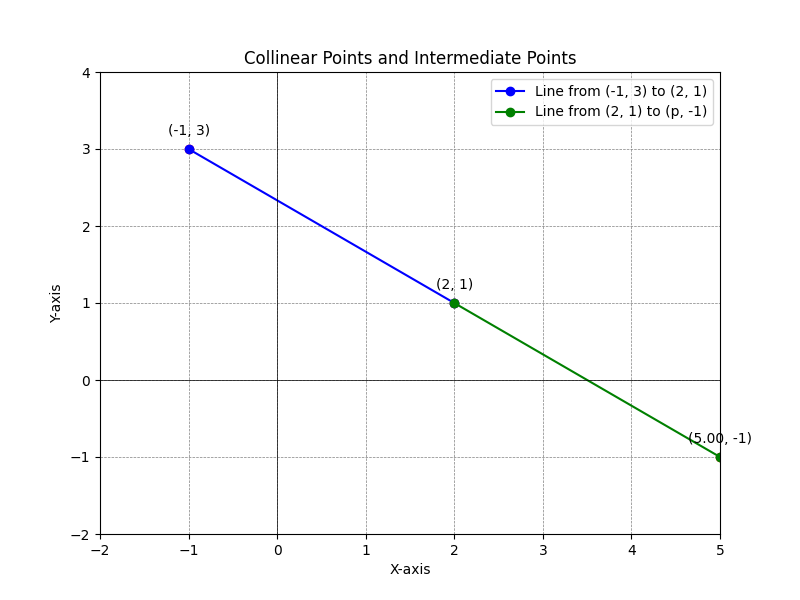
\includegraphics[width=0.8\textwidth]{figs/fig.png}
	\caption{A plot of the given question.}
	\label{fig:Plot1}
\end{figure}
\end{frame}
\subsection{Code}
\begin{frame}[fragile,allowframebreaks]
\lstset{
        language = C,
        basicstyle=\ttfamily\tiny,
        keywordstyle=\color{blue},
        stringstyle=\color{green},
        commentstyle=\color{gray},
        tabsize=4
    }
    \lstinputlisting{./codes/collinear.c}
\end{frame}
\subsection{Code}
\begin{frame}[fragile,allowframebreaks]

\lstset{
        language = Python,
        basicstyle=\ttfamily\tiny,
        keywordstyle=\color{blue},
        stringstyle=\color{green},
        commentstyle=\color{gray},
        tabsize=4
    }
    \lstinputlisting{./codes/plot.py}
\end{frame}


\end{document}

